\section{Konfidenzintervall}
  \subsection{Begriffe}
   Irrtumswahrscheinlichkeit = $ \alpha $; 
  Konfidenzniveau =  $ 1-\alpha = $ ; 
  Konfidenzintervall = $ I $
  \subsection{Punkschätzer}
  E[X]: Stichprobenmittel:
  $ \overline{X = \frac{1}{n}} \sum_{i=1}^{n} X_{i}$; 
  Varianz: Stichprobenvarianz:
  $ s^{2} = \frac{1}{n -1} \sum_{i=1}^{n} (X_{i} - \overline{X})^{2} $; 
  Schätzwert für wahren Parameter, aber keine Aussage über Unsicherheit der Schätzung, Geringe Sicherheit für wahren Parameter; 
  
  \subsection{Intervallschätzer}
  Intervall für wahren Parameter, mit vorgegebener Sicherheit; Vorgabe (95\% or 99\%); 
  Dichtefunktion:
  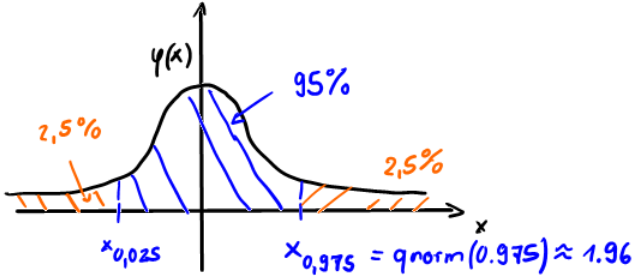
\includegraphics[scale=0.25]{./pic/KonfidenzintervallDichtefunktion.png}
  $ P(-a \le \overline{x} \le a) > 0.95 $; 
  $ \sigma ist $ unbekannter Parameter\\
  $ P( x_{\underbrace{0.025}} < \underbrace{ \frac{\overline{x} - \mu}{\sigma}\sqrt{n} } < x_{\underbrace{0.975}} ) \ge 0.95 $\\
  $ -1.96; N_{0,1}; 1.96 $; 
  
  \subsection{$ \mu $, unbekannt, $ \sigma^{2} $, bekannt}
  $ I = ] \overline{X} \textbf{-} \underbrace{\phi^{-1}( 1-\frac{\alpha}{2} ) } \frac{\sigma}{ \sqrt{n} }\textbf{,} $\\ 
  $ qnorm ( 1-\frac{\alpha}{2} ) $\\
  $ \overline{X} \textbf{+} \phi^{-1} ( 1- \frac{\alpha}{2} ) \frac{\sigma}{ \sqrt{n} } [ $; 
  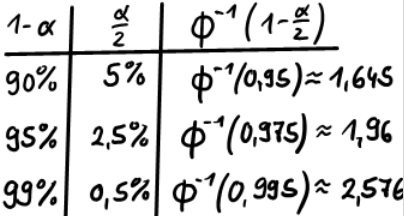
\includegraphics[scale=0.25]{./pic/QnormTabelle.png}
  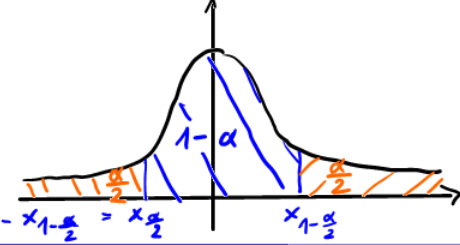
\includegraphics[scale=0.25]{./pic/KonfidenzintervallDichtefunktionTabelle.png}

  \subsection{$ \mu $ \& $ \sigma^{2} $, unbekannt }
  $ I = ] \overline{X} \textbf{-} t_{n-1}^{-1} ( 1-\frac{\alpha}{2} ) \frac{S}{ \sqrt{n} } \textbf{,} \overline{X}  \textbf{+} t_{n-1}^{-1} ( 1-\frac{\alpha}{2} )\frac{S}{ \sqrt{n} } [ $
  